\section{Arquitectura de Software:}
    Para la implementación del sistema se utilizó el patrón de diseño de Software MVC. 
    \subsection{MVC}
    MVC (Modelo-Vista-Controlador) es un patrón en el diseño de software comúnmente utilizado para implementar interfaces de usuario, datos y lógica de control. Enfatiza una separación entre la lógica de negocios y su visualización. Esta "separación de preocupaciones" proporciona una mejor división del trabajo y una mejora de mantenimiento
    Las tres partes del patrón de diseño de software MVC se pueden describir de la siguiente manera:
    \begin{itemize}
        \item Modelo: Maneja datos y lógica de negocios.
        \item Vista: Se encarga del diseño y presentación.
        \item Controlador: Enruta comandos a los modelos y vistas.
    \end{itemize}
    \begin{figure}[H]
		\centering
		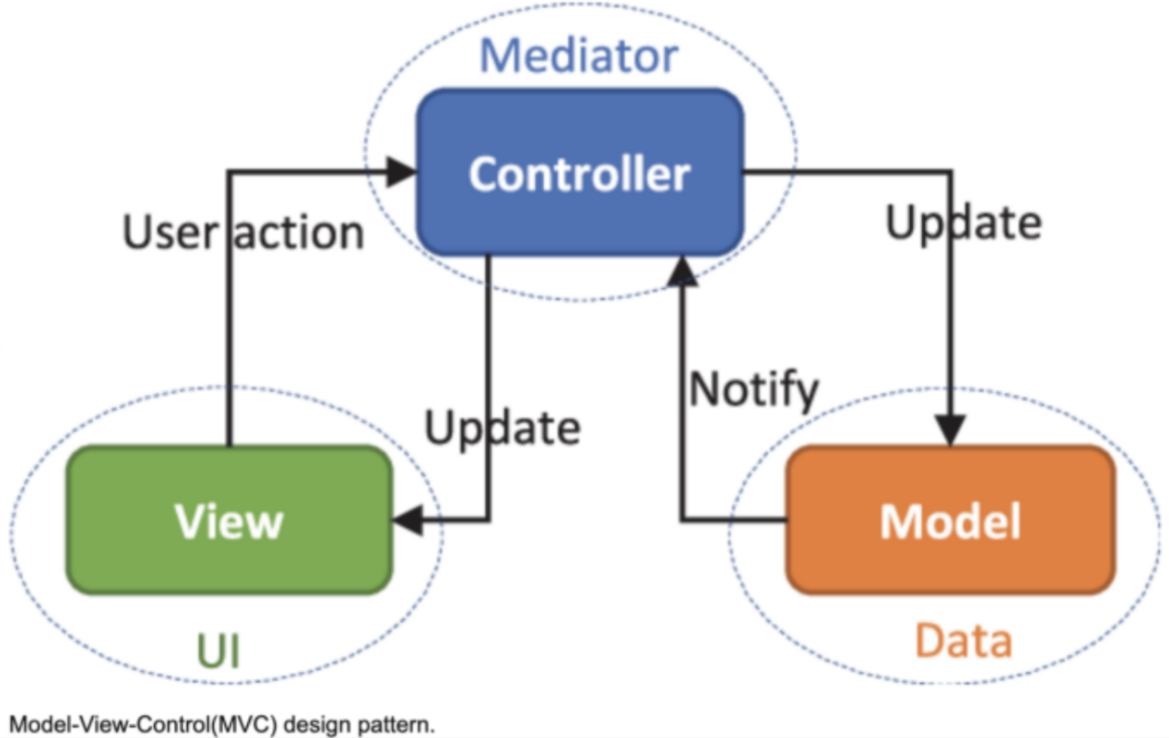
\includegraphics[width=\textwidth,height=\textheight,keepaspectratio]{Extras/MVC}
		\caption{Modelo-Vista-Controlador}
		\label{fig:MVC}
	\end{figure}

    